%%This is a very basic article template.
%%There is just one section and two subsections.
\documentclass{article}

% use Times
\usepackage{times}

\usepackage{amsmath,amssymb, amsthm}
%\usepackage{charter}
%\usepackage{calc}


%\usepackage{multirow}
%\usepackage[cp1250]{inputenc}
%\usepackage[T1]{fontenc}
%\usepackage{calligra}
%\usepackage[slovak]{babel}
\usepackage{amsfonts}
\usepackage{layout}
\usepackage{amsmath}
\usepackage{amsthm}
\usepackage{amssymb}

%\usepackage[dvips]{graphicx}
\usepackage{url}
\usepackage{color}
\usepackage{graphicx}
%\usepackage{algorithmic}
%\usepackage{algorithm}
\usepackage{verbatim}



\newcommand{\del}[1]{{\color{red}{#1}}}

\let\la=\langle
\let\ra=\rangle

\newcommand{\st}{\;:\;}
\newcommand{\ve}[2]{\langle #1 ,  #2 \rangle}

\newcommand{\pseudoinv}[1]{#1^{-1}}

\newcommand{\eqdef}{\stackrel{\text{def}}{=}}

\newcommand{\ii}{{}^{(i)}}

\newcommand{\R}{\mathbb{R}}
\newcommand{\Prob}{\mathbf{Prob}}
\newcommand{\E}{\mathbf{E}}


\newcommand{\pc}[2]{#1^{[#2]}}

\newcommand{\vc}[2]{#1^{(#2)}}

\newcommand{\vs}[2]{#1_{[#2]}}


\newcommand{\nc}[2]{{\|#1\|_{(#2)}}}
\newcommand{\ncs}[2]{\|#1\|^2_{(#2)}}
\newcommand{\ncc}[2]{{\|#1\|^*_{(#2)}}}
\newcommand{\ls}[1]{{\mathcal S(#1)}}
\newcommand{\Rw}[2]{\mathcal R_{#1}(#2)}
\newcommand{\Rws}[2]{\mathcal R^2_{#1}(#2)}

\newcommand{\Rel}[2]{\mathcal {R}_{#1}^{#2}}


\newcommand{\nbp}[2]{\|#1\|_{(#2)}}   % norm block primal
\newcommand{\nbd}[2]{\|#1\|_{(#2)}^*} % norm block dual

\newcommand{\lf}{\mathcal L}
\newcommand{\U}{\mathbf U}
\newcommand{\bU}{\mathbf U}
\newcommand{\B}{\mathbf B}
\newcommand{\bA}{\mathbf A}
\newcommand{\bB}{\mathbf B}
\newcommand{\bM}{\mathbf M}
\newcommand{\bE}{\mathbf E}
\newcommand{\bI}{\mathbf I}
\newcommand{\bH}{\mathbf H}
\newcommand{\bG}{\mathbf G}
\newcommand{\bS}{\mathbf S}
\newcommand{\cS}{\mathcal{ S}}
\newcommand{\pP}{\mathcal{P}}
\newcommand{\N}{N}

\newcommand{\mLi}{{m^{(i)}}}
\newcommand{\gLi}{{g^{(i)}}}
%\newcommand{\TLi}{{\color{red}T_L^{(i)}}}
\newcommand{\TLi}[1]{{T^{(#1)}}}
\newcommand{\TL}{{T}}

\DeclareMathOperator{\support}{{support}}

\DeclareMathOperator{\mynnz}{{nnz}}
\DeclareMathOperator*{\argmin}{\arg\min}
\DeclareMathOperator*{\argmax}{\arg\max}

\newcommand{\Lip}{L}
\newcommand{\ALip}{\tilde L}

\newcommand{\Rc}[1]{{\mathbf{RC}_{(#1)}}}
\newcommand{\NRCDM}{{NRCDM}\  }
\newcommand{\nnz}[1]{{\|#1\|_0}}
% sets
\DeclareMathOperator{\card}{card}       % cardinality of a set
\DeclareMathOperator{\diam}{diam}       % diameter of a set
\DeclareMathOperator{\MVEE}{MVEE}       % minim volume enclosing ellipsoid of a set
\DeclareMathOperator{\vol}{vol}         % volume of a set

% statistical
\DeclareMathOperator{\Exp}{\mathbb{E}}           % expectation
\DeclareMathOperator{\Cov}{Cov}         % covariance
\DeclareMathOperator{\Var}{Var}         % variance
\DeclareMathOperator{\Corr}{Corr}       % correlation

% functions and operators
\DeclareMathOperator{\signum}{sign}     % signum/sign of a scalar
\DeclareMathOperator{\dom}{dom}         % domain
\DeclareMathOperator{\epi}{epi}         % epigraph
\DeclareMathOperator{\Ker}{null}        % nullspace/kernel
\DeclareMathOperator{\nullspace}{null}  % nullpsace
\DeclareMathOperator{\range}{range}     % range
\DeclareMathOperator{\Image}{Im}        % image

% topology
\DeclareMathOperator{\interior}{int}    % interior
\DeclareMathOperator{\ri}{rint}         % relative interior
\DeclareMathOperator{\rint}{rint}       % relative interior
\DeclareMathOperator{\bdry}{bdry}       % boundary
\DeclareMathOperator{\cl}{cl}           % closure

% vectors, matrices
\DeclareMathOperator{\linspan}{span}
\DeclareMathOperator{\linspace}{linspace}
\DeclareMathOperator{\cone}{cone}

\DeclareMathOperator{\trace}{tr}           % trace
\DeclareMathOperator{\tr}{tr}           % trace
\DeclareMathOperator{\rank}{rank}       % rank
\DeclareMathOperator{\conv}{conv}       % convex hull
\DeclareMathOperator{\Diag}{Diag}       % Diag(v) = diagonal matrix with v_i on the diagonal
\DeclareMathOperator{\diag}{diag}       % diag(D) = the diagonal vector of matrix D

\DeclareMathOperator{\Arg}{Arg}         % Argument
% the * at the end of operator seems to have the effect that the command will be properly have its sub/superstripts vertically below/above it, like \sum for example, this only applies if you are in \displaystyle
\DeclareMathOperator{\lmax}{\lambda_{\max}}
\DeclareMathOperator{\lmin}{\lambda_{\min}}
\DeclareMathOperator*{\supp}{supp}
\DeclareMathOperator*{\sign}{sign}
\DeclareMathOperator*{\rk}{Rk}
\DeclareMathOperator*{\relint}{\mathop{relint}}

%norms
\providecommand{\abs}[1]{\left\lvert#1\right\rvert}
\providecommand{\norm}[1]{\left\lVert#1\right\rVert}

\newcommand{\ball}{\mathcal{B}}
\newcommand{\sphere}{\mathcal{S}}

\newcommand{\bigO}{O}
\newcommand{\X}{\mathcal{X}}
\newcommand{\Sym}{\mathcal{S}}
\newcommand{\Supt}{\Sym_{(t)}}
\newcommand{\Suptc}{\bar{\Sym}_{(t)}}
%\renewcommand{\qedsymbol}{\ding{114}}


\newtheorem{algorithms}{Algorithm}

\newtheorem{example}{Example}

\theoremstyle{plain}
\newtheorem{theorem}{Theorem}
\newtheorem{proposition}[theorem]{Proposition}
\newtheorem{corollary}[theorem]{Corollary}
\newtheorem{lemma}[theorem]{Lemma}
\newtheorem{claim}[theorem]{Claim}
\newtheorem{remark}[theorem]{Remark}
\newtheorem{assumption}[theorem]{Assumption}
\newtheorem{assump}[theorem]{Assumption}


\theoremstyle{definition}

\newtheorem{exercise}[theorem]{Exercise}

\newtheorem{rem}[theorem]{Remark}
\newtheorem{que}[theorem]{Question}
\newtheorem{definition}[theorem]{Definition}
 
\newcommand{\appcof}{v}
\newcommand{\domain}{\mathcal{D}}

\newcommand{\points}{\mathcal{A}}
\newcommand{\stepsize}{\gamma}
\newcommand{\Cf}{C_{\hspace{-0.08em}f}}
\newcommand{\x}{\bm{x}}
\newcommand{\g}{\bm{g}}
\newcommand{\G}{{\cal G}}
\newcommand{\I}{\mathbb{I}}
\newcommand{\y}{\bm{y}}
\newcommand{\z}{\bm{z}}
\newcommand{\s}{\bm{s}}
\newcommand{\shat}{\bm{\hat{s}}}
\newcommand{\bv}{\bm{b}}
\newcommand{\dv}{\bm{d}}
\newcommand{\qv}{\bm{q}}
\newcommand{\uv}{\bm{u}}
\newcommand{\av}{\bm{v}}
\newcommand{\vv}{\bm{v}}
\newcommand{\w}{\bm{w}}
\newcommand{\xv}{\bm{x}}
\newcommand{\row}{\text{row}}
\newcommand{\col}{\text{col}}
\newcommand{\lft}{\text{left}}
\newcommand{\rgt}{\text{right}}
\newcommand{\dualp}{\bm{\alpha}}
\newcommand{\risk}{{\cal R}}
\newcommand{\signVec}{\mathbf{s}}
\newcommand{\F}{\mathbb{F}}
\newcommand{\M}{\mathbb{M}}
\newcommand{\id}{\mathbf{I}} % big i for identity
\newcommand{\ind}{\mathbf{1}} % indicator vectors
\newcommand{\0}{\mathbf{0}} % the origin
\newcommand{\unit}{\mathbf{e}} % unit basis vectors
\newcommand{\one}{\mathbf{1}} % all one vector
\newcommand{\zero}{\mathbf{0}}
\newcommand\SetOf[2]{\left\{#1\vphantom{#2}\right.\left|\vphantom{#1}\,#2\right\}}
\newcommand{\ignore}[1]{}%{\textbf{***begin ignore***}\\#1\textbf{***end ignore***}}
\newcommand{\bound}{{\cal H}}
\renewcommand{\S}{{\cal S}}
\newcommand{\T}{{\cal T}}
\newcommand{\C}{{\cal C}}

\newcommand{\idea}[1]{\marginpar[\hspace*{4.5em}\textbf{IDEA}\hspace*{-4.5em}]{\textbf{IDEA}}\textbf{IDEA:}
#1}
\newcommand{\note}[1]{\marginpar{#1}}

\newcommand*{\rom}[1]{\expandafter\@slowromancap\romannumeral #1@}

% For figures
\usepackage{graphicx} % more modern
%\usepackage{epsfig} % less modern
\usepackage{subfigure} 
\usepackage[colorinlistoftodos,bordercolor=orange,backgroundcolor=orange!20,linecolor=orange,textsize=scriptsize]{todonotes}

% For citations
\usepackage{natbib}

 \usepackage{graphicx}
\usepackage{epsfig}
\usepackage{epstopdf}
\graphicspath{ {./images/} }
\usepackage{hyperref}
\usepackage{bm,color}
\usepackage{verbatim}
\usepackage{wrapfig}
\usepackage{caption}

\usepackage{tikz}
\usepackage{tkz-euclide}
\usetkzobj{all}
\usepackage[boxruled,commentsnumbered]{algorithm2e}
\usepackage{booktabs}



% the only way to get two column algorithms seems to be to use a hack on top of the algorithm2e package
\usepackage{multicol}
%\usepackage[ruled,commentsnumbered]{algorithm2e}

\newenvironment{algo}{%
  \renewenvironment{algocf}[1][h]{}{}% pass over the floating stuff
  \algorithm
}{%z
  \endalgorithm
}

\definecolor{darkgreen}{rgb}{0,.4,.2}
\definecolor{darkblue}{rgb}{.1,.2,.6}
\definecolor{brightblue}{rgb}{0,0.6,0.8}
\hypersetup{
  colorlinks=true,
  linkcolor=darkblue,
  citecolor=darkgreen,
  filecolor=darkblue,
  urlcolor=darkblue
}
\usepackage{pifont}% http://ctan.org/pkg/pifont
\newcommand{\cmark}{\ding{51}}%
\newcommand{\xmark}{\ding{55}}%
\newcommand{\smoothstrong}{\S_{\mu,L}^{1,1}}
\usepackage{scalerel,stackengine}
\stackMath
\newcommand\reallywidehat[1]{%
\savestack{\tmpbox}{\stretchto{%
  \scaleto{%
    \scalerel*[\widthof{\ensuremath{#1}}]{\kern-.6pt\bigwedge\kern-.6pt}%
    {\rule[-\textheight/2]{1ex}{\textheight}}%WIDTH-LIMITED BIG WEDGE
  }{\textheight}% 
}{0.5ex}}%
\stackon[1pt]{#1}{\tmpbox}%
}
\newcommand{\ERM}{\widehat{\w}_n}
\newcommand{\opt}{\w^*}

\usepackage{amsmath}
\usepackage{nips15submit_e,times}
\author{}




\begin{document}
\title{Learning with Adaptive Sample Sizes}

%\author{\\ Author Name\\
%{\small \href{mailto:author@ethz.ch}{author@ethz.ch}}}
\date{} 

\maketitle

\section{Problem Setting}
\subsection{Empirical Risk Minimization}
We assume that there is some (unknown) distribution $P$ that generates samples
$\x \sim P$. For a given training set $\T = \{\x_i: \x_i \sim P \}$, we denote
the empirical risk (ER) and its minimizer by
\begin{align}
\risk_\T(\w) := \frac {1}{|\T|} \sum_{\x \in \T} f_{\x}(\w),
\qquad \w^*_\T := \argmin_{\w} \risk_{\T}(\w) 
\end{align}
Moreover, we define the expected risk of a parameter as $\risk(\w) := \E
f_{\x}(\w)$ and its minimum and minimzer by $\risk^*$ and $\w^*$, respectively.
Since the distribution $P$ is unknown, empirical risk minimization approach
uses empirical minimizer $\w_n = \arg\min_{\w} \risk_{\T}(\w)$ to estimate
$\w^*$. In later section, we will mention the depedency of empirical risk
minimizer (ERM) to expected risk minimizer. Nonethless, our focus is on
empirical risk throughout this section. The following conditions
on empirical risk underlie in our analysis:
\begin{itemize}
  \item \textbf{$\mu$-strong convexity:} we assume for all sufficiently large
  sample size $\forall \T:|\T|> \T_0$, the empirical risk is $\mu$-strongly
  convex with high probability, which means: 
  \begin{equation*}
  	\langle \nabla \risk_\T(\w_1) - \nabla \risk_\T(\w_2), \w_1 - \w_2 \rangle
  	\geq  \mu \| \w_1 - \w_2 \|_2^2
  \end{equation*}
  \item \textbf{Partial $L$-smoothness:} This assumption indicates that the
  gradient of each summand of empirical risk is $L$-Lipschitz. Note that this
  assumption is stronger than the $L$-smoothness assumption on the empirical
  risk.
  \begin{equation*}
  	\| \nabla f_{\x}(\w_1) - \nabla f_{\x}(\w_2) \|_2
  	\leq  L \| \w_1 - \w_2 \|_2
  \end{equation*}
  \item \textbf{Continuity:} The domain $\domain[\risk_\T(\w_1)]$ spans
  $\R^d$ and it is continous on this domain. Furthermore, its gradient exists on
  all domain. 
\end{itemize}
Let $\smoothstrong$ denote all empirical risks
 for which above conditions hold. The following lemma holds for
all functions $f(\w) \in \smoothstrong$. 
\begin{lemma}
	Assume function $f(\w) \in \smoothstrong$, then for all $\w_1$ and $\w_2$ the
	following inequality holds: 
    \begin{equation*}
    	| f(\w_1) - f(\w_2) - \langle \nabla f(\w_2), \w_1 - \w_2 \rangle | \leq
    	L \| \w_1 - \w_2 \| ^2 
    \end{equation*}
\end{lemma}
\begin{proof}
	The proof is provide by \cite{nesterov2004introductory} (Lemma 1.2.3). However
	we provide a simpler proof here to keep the consistancy. Based on the ``Mean
	Value Theorem'', there is a $\w_{\tau} = \w_2 + \tau(\w_1-\w_2), \tau \in [0,1]$
	that satisfies:
	\begin{equation*}
		f(\w_1) - f(\w_2) = \langle \nabla f(\w_{\tau}), \w_1 - \w_2 \rangle
	\end{equation*}
	Pluging the above equation inside the left side of inequality, yields: 
	\begin{eqnarray*}
		& | f(\w_1) - f(\w_2) - \langle \nabla f(\w_2), \w_1 - \w_2 \rangle | \\ 
		& = | \langle \nabla f(\w_{\tau}) - \nabla f(\w_2), \w_1 - \w_2 \rangle| \\ 
		& \leq \|  \nabla f(\w_{\tau}) - \nabla f(\w_2) \| \|\w_1 - \w_2 \|
		\\
		& \leq L \|  \w_{\tau} - \w_2 \| \|\w_1 - \w_2 \| \leq L \|\w_1 -
		\w_2 \|^2 \\
	\end{eqnarray*}
	The third and forth steps are achieved by Cauchy-Schwarz inequality and the
	$L$-smoothness assumption, respectively. 
\end{proof}
\begin{corollary} \label{corollary:smoothstrongbound}
	Let $f(\w) \in \smoothstrong$ and $f^*$ and $\w^*$ denote its minimum and
	minimal, then: 
	\begin{equation*}
		\frac{\mu}{2} \| \w - \w^*  \| \leq f(\w) - f^* \leq L \| \w - \w^* \|^2
	\end{equation*}
\end{corollary}
\begin{proof}
	The left side inequality is direct result of $\mu$-strong convexity
	assumption and the optimality of $\w^*$. The right side is achieved by
	the last Lemma.
\end{proof}

\subsection{Generalization bound}
Generalization bounds aim at uniformly bounding the deviation between the empirical and the expected risk over the function class at hand. A typical bound takes the form
\begin{equation*}
\E_\T \left[ \sup_{\w} \left| \risk(\w) - \risk_\T(\w) \right| \right]  \leq
\bound(n) \label{eq:bound}
\end{equation*} 
where the expectation is over a random sample $\T$ of fixed size $|\T|=n$. 
Here $\bound$ is a bound that depends on $n$, usually in a ratio $n/d$ relative to some capacity measure $d$ 
of the function class (e.g.~in the linear case the dimensionality or the VC dimension), which we assume to be constant in our discussion.  
A simple, often conservative bound may scale as $\bound(n) \in \bigO(1/\sqrt{n})$. 
It is sometimes possible to derive more optimistic bounds on the estimation accuracy (e.g.~in the realizable case) 
such as $\bound(n) \in \bigO(\log(n)/n)$ or even $\bound(n) \in\bigO(1/n)$. 
 Surprsingly, our proposed convergence does depend on the generalization bound.
 Indeed, we consider two cases for the convergence rate: 
 \begin{itemize}
   \item \textbf{GERM: } General Uniform Convergence rate of ERM
  means when  $\bound(n) =
   \bigO\left(\frac{1}{\sqrt{n}}\right)$. 
   \item \textbf{FERM: }Fast Uniform Convergence rate of ERM
   is order of $\bound(n) = \bigO \left( \frac{1}{n} \right)$ 
 \end{itemize}
 
Note that the bounds hold with high probability over the choice of the sample set. So there could always be sample sets that violate the bound. Morever, the uniform convergence (supremum over all solutions $\w$) is required to allow dependencies between $\w$  and the (random) data. It holds in particular it holds for $\w$ that are minimizer of empirical risks or approximations thereof. 
Assume we have some solution $\w_\T$ that is (by design) guranteed to be an
$\epsilon$-approximation in the empirical risk, namely $\risk_\T(\w_\T) - \risk_\T^* \le \epsilon$.
 We can bound its $P$-suboptimality in expectation over the random choice of $\S$ as follows 
\begin{align}
\label{eq:exprisk-bound}
\E \risk(\w_\T) - \risk^*  & = 
\E \left[ \risk(\w_\T) \mp \risk_{\T}(\w_{\T}) \mp \risk_{\T}(\w_{\T}^*) \mp
\risk_\T(\w^*) \right]   - \risk(\w^*)
% \\  & \le \E \sup_\w \{ | \risk(\w) -  \risk_\S(\w) | \} + \epsilon + 0 + \E \risk_\S(\w^*) - \risk(\w^*) 
\\ & \le \E \sup_{\w} \{ | \risk(\w) -  \risk_\T(\w) | \} + \epsilon  \le 
\bound(n) + \epsilon
\nonumber
\end{align}
This means, we can basically add up bounds on the statistical accuracy and the
optimization error. 
We aim at proposing an optimization method which iteratively increase the size
of training set. In this manuscript, we very often need to translate the
suboptimality on a subsample of the training set to suboptimality on empirical
risk of the training set. To this end, we will frequently use the following
Theorem.
 \begin{theorem} \label{theorem:generalization_bound_on_subset}
 		Let $\w_\S$ is $\epsilon$-suboptimal on sample $\S$, means 
 		$\risk_\S(\w_\S) - \risk_\S^* \le \epsilon$. 
 		If $\S \subset \T$ is a subset of $\T$, then suboptimality of $\w_\S$ on set
 		$\T$ is bounded w.h.p as: 
 		\begin{align}
			\E \left[ \risk_\T(\w_\S) - \risk_\T^*\right] \le \epsilon +
			\frac{|\T|-|\S|}{|\T|} \bound(|\S|)
			\label{eq:new-epsilon} 
		\end{align}
		where expecation is over random choice of set $\T$. 
 \end{theorem}
\begin{proof}
For simplicity we use notations $N = | \T |$ and $n = | \S |$ in the proof.
Clearly, $N > n$ holds. We consider the chain:
\begin{align}
\risk_\T(\w_\S) - \risk_\T^* = \risk_\T(\w_\S) \stackrel{[1]}{\mp} \risk_\S(\w_S) \stackrel{[2]}{\mp} \risk_\S(\w_\S^*) \stackrel{[3]}{-} \risk_\T(\w_\T^*)
\end{align}
We bound the three involved differences as follows: 
\begin{align}
\text{[2]} \quad & \risk_\S(\w_S)  - \risk_\S(\w_\S^*) \le \epsilon  \qquad 
\text{($\epsilon$ optimality of $\w_\S$ with regard to $\risk_\S$)}
\\
\text{[3]} \quad & \E_\T \left[ \risk_\S(\w_\S^*) - \risk_\T(\w_\T^*) \right] \le 0 \qquad 
\text{(optimizing over a subsample)}
% \\
%& \E_\T \left[ \risk_\S(\w_\S^*) - \E_{\T} \risk_\T(\w_\S^*) \right] \le 0 \qquad 
%\text{(since $\E\risk_\S(\w^*_\S) \le \risk(\w_\S)$)}
\end{align}
The latter inequality can be justifed by
\begin{align}
\E_{\S} \risk_\S(\w_\S^*) \stackrel{[4]}{\le} \E_{\T} \risk_\S(\w_\T^*)  \stackrel{[5]}= \E_{\T} \risk_\T(\w_\T^*)  
\end{align}
where 
\begin{align}
\text{[4]} \quad & \risk_\S(\w_\S^*) \le \risk_\S(\w), \quad \forall \w\\
\text{[5]} \quad & \E_{\S | \T} \risk_\S(\w) = \risk_\T(\w), \quad \forall \w \quad \text{as $\S \subset \T$}
\end{align}
Moreover, we have that
\begin{align}
& \E_{\T-\S} \left[ \risk_\T(\w_\S) - \risk_\S(\w_S) \right] \le \frac{N- n}{N} | \risk(\w_S) - \risk_\S(\w_\S) |
\label{eq:t-s} \qquad 
\end{align}
The above inequlity might seems a bit complicate to prove this we follow as: 
\begin{eqnarray*}
  & \E_{\T-\S} \left[ \risk_\T(\w_\S) - \risk_\S(\w_S) \right] & = \E_{\T-\S}
  \left[
  \frac{1}{N} \left[  \sum_{\x \in \S} f_{\x}(\w_\S)  + \sum_{\y \in \T - \S}
  f_{\y}(\w_\S)\right] - \frac{1}{n}  \sum_{\x \in \S} f_{\x}(\w_\S)  \right]\\
  & & =  
  \frac{N-n}{N} \E_{\T-\S} \left[ \frac{1}{N-n} \sum_{\y \in \T - \S}
  f_{\y}(\w_\S) -  \risk_\S(\w_{\S}) \right] \\
  & & = \frac{N-n}{N} \E_{\T-\S} \left[ \frac{1}{N-n} \sum_{\y \in \T - \S}
  f_{\y}(\w_\S) -  \risk_\S(\w_{\S}) \right]\\ 
  & &  = \frac{N-n}{N}\left[ \E_{\T-\S} \left[ \risk_{\T-\S}(\w_\S) \right]-
  \risk_\S(\w_{\S}) \right] \\ 
  & & = \frac{N-n}{N} \left[\risk(\w_{\S}) - \risk_\S(\w_{\S})\right]
\end{eqnarray*}

and hence 
\begin{align}
\text{[1]} \quad & \E_{\T} \left[ \risk_\T(\w_\S) - \risk_\S(\w_S) \right] \le
\frac{N-n}{N} \sup_{\w} | \risk(\w) - \risk_\S(\w) | \le \frac{N-n}{N} \bound(n)
\label{eq:t-s-all} 
\end{align}
The inqualities [1], [2], and [3] conclude the suboptimality bound. 
\end{proof}

\subsection{First order oracle computational complexity} 
Here, we aim at proposing a new ``Incremental First Order Method'' (IFOM)
\cite{agarwal2015lower}. Given a the training set $|\T| = n $, IFOM optimizes
the empirical risk troughout computing stochastic gradients on a point $\x_i \in
\T, i \in \{ 1,\ldots, n \}$, which is defined as: 
\begin{equation*}
	\nabla_{\x_i} \risk_{\T}(\w) = \nabla f_{\x_i} (\w)
\end{equation*} 
Note that the gradient of empirical is indeed the expected value of the
stochastic gradient means:
\begin{equation*}
	\nabla \risk_{\T}(\w) = \E_{\x_t \sim P(\T)} \left[\nabla_{\x_i}
	\R_{\T}(\w)\right],
\end{equation*}
where expectation is over the empirical distribution over the training set
i.e. $P(\T)$.
Our setting is restricted to computation of the stochastic gradient for at most
$\C$ times. Indeed, we consider each computation of stochastic gradient as a unit of
computational complexity. Note that computation of stochastic
gradient needs $\bigO(d)$ computational complexity. But in our regim, where $n
\gg d$, we consider $d$ as a constant. 
For example, SAGA yields the following
suboptimality using $\C$ oracle computational budget \cite{defazio2014saga} as
long as $\risk_{\T} \in \smoothstrong$:
\begin{equation*}
	\E_{\x_{\C}}\| \w_{\C} - \w^*_{\T} \|^2 \leq \rho_{n}^{\C} \epsilon_0,
\end{equation*}
where $n = | \T |$, and $\epsilon_0$ denotes the initial error that
depends on the initial parameter.

 Here, $\rho_{n}$ is the convergence factor, which is defined as:
\begin{equation*}
	\rho_n = 1- \min\left\{ \frac{1}{4n}, \frac{\mu}{3 L} \right\}
\end{equation*}
We can translate this suboptimality in terms of risk using Lemma
\ref{corollary:smoothstrongbound}. More precisely,
\begin{equation*}
	\risk_{\T}( \w_{\C}^+) - \risk^*_{\T} \leq L \rho_{n}^{\C} \epsilon_0
\end{equation*}

 Consider the setting where
the convergence factor is dominated by the sample size, means $\rho_n = \frac{1}{n}$. In this case, there is a caveat
regarding the convergence rate $\rho_n$:
in the large-scale setting, where $n$ goes to infinity, the convergence rate
slows down. Here, we aim at tackling this issue.
\section{Motivation} 
Consider the setting where the convergence factor $\rho_n$ is dominated by
size of traing set i.e. $\rho_n = \bigO\left(\frac{1}{n}\right)$. As mentioned
in the last section, SAGA results an unfovarable convergence factor $\rho_n \to 1$ in this
setting.
Here, we aim at improving the convergence of SAGA in the large-scale setting. We
demonstrate the idea with a simple example; assume our traing set has size $|\T|
= n$, and our computational oracl complexity is limited to $\C = n$, which means
we are allowed to do one pass over the training set.
 If we pick all the traing set $\T$, then SAGA garantees the following
 convergence rate:
 \begin{equation*}
 	\E_{\x_{n}} \left[\risk_{\T}( \w_{\T}^+) - \risk^*_{\T}\right] \leq 
 	(1-\frac{1}{n})^n L \epsilon_0 \leq \exp(-1) L\epsilon_0
 \end{equation*}
However, we can achieve a better suboptimality bound using the same method i.e.
SAGA. If we randomly sample half of the data $\S \subset \T$, such that $|\S| =
\frac{n}{2}$, and iterate on it for $n$ times, then we can provide a better
suboptimal solution on the risk $\risk_{\S}$: 
\begin{equation*}
	\E_{\x_{n}} \left[ \risk_{\S}( \w_{\S}^+) - \risk^*_{\S}\right] \leq (1-
	\frac{n}{2}) ^n L \epsilon_0 \leq \exp(-2) L \epsilon_0'
\end{equation*}
We assume the initial error is the same for both small and large set i.e.
$\epsilon_0 = \epsilon_0'$. Theorem
\ref{theorem:generalization_bound_on_subset} states we can translate the bound
to the suboptamility of risk on the superset $\T$ by paying additional cost: 
\begin{equation*}
	\E_{\x_n, \T} \left[\risk_{\T} (\w_{\S}^+) - \risk^*_{\T} \right] \leq 
	\exp(-2) L \epsilon_0 + \frac{1}{2} \bound(\frac{n}{2})
\end{equation*}
where the expection is over the random choice of $\x_n$, as the stochastic
gradient pivot, and random choice of all training set with size $n$ i.e.
$\forall |\T| = n$. The additional cost $\frac{1}{2} \bound(\frac{n}{2})$ is
relatively small for considerably large data set, when $\bound(n/2)<2 \exp(-1) L\epsilon_0$ holds.
	Therefore, SAGA surperisingly yields a better
	suboptimality using a smaller set, as it is illusterated in Figure
	\ref{fig:geometric}. This motivates us to propose an adaptive sample size
	strategy for SAGA.
	In other words, we aim at staring the optimization on a smaller subset of
	the data and iteratively increase the size of the optimization set.
	Our analysis will show that adaptive sample size SAGA enjoys a better convergenc rate. 
\begin{figure}
    \begin{center}
        \begin{tikzpicture}[thick]
        \node (O) at (0,0) {\textbullet};%x
        \node (B) at (5,5) {\textbullet};%xs
        \coordinate (D) at (0,-3);%rn
        \node (E) at (-2,2) {\textbullet};%xm
        \node (G) at (4,4){\textbullet};%wpn
        \node (H) at (1.5,3.5){\textbullet};%wpm
        \draw [dashed] (B)--(O);
        \draw [dashed] (B)--(E);
        \draw  [dashed] (O) circle (3cm);
        \draw  [dashed]  (O)--(D);
        \draw [->] (B)--(G);
        \draw [->] (B)--(H);
        \tkzLabelSegment[below=2pt](O,O){\textit{$\risk_{\T}^*$}}
        \tkzLabelSegment[below=2pt](G,G){\textit{$\w^+_{\T}$}}
        \tkzLabelSegment[below=2pt](H,H){\textit{$\w^+_{\S}$}}
        \tkzLabelSegment[below=2pt](E,E){\textit{$\risk_{\S}^*$}}
        \tkzLabelSegment[below=2pt](O,O){\textit{$\risk_{\T}^*$}}
        \tkzLabelSegment[above=2pt](B,B){\textit{$\w_0$}}
        \tkzLabelSegment[left=2pt](O,D){\textit{$\frac{1}{2}\bound(\frac{n}{2})$}}
        \end{tikzpicture}
    \end{center}
    \caption{SAGA enjoys a better convergence rate on a smaller training set
    $\S \subset \T$; here $|\T| = n$ and $|\S| = \frac{n}{2}$. }
  \label{fig:geometric}
\end{figure}
\section{Adaptive sample size method}
Now, we are ready to introduce the adaptive sample size startegy. We are given
computational budget $\C$, the training set $|\T| = n$, the risk function
$\risk_{\S} \in \smoothstrong$, and SAGA optimization method.  Let
$\U\left(\C,\T\right)$ denote the best achievable suboptimaily upper-bound on
the empirical risk $\risk_{\T}$, which is induced by the set $\T$, using the
limited computational complexity $\C$ and SAGA method.
\begin{equation*}
	  \min_{\w_{\C}} \E_{\x_{\C}, \T}| \risk_{\T}(\w_{\C}) - \risk_{\T}^* | \leq
	  \U(\C,\T)
\end{equation*} 
where the expecation is with respect to both random choice of the training point
and random choice of set $\T$. 
\todo[inline]{ We have to work on this notation more. For example when $\T$ is
the whole training set, then expecation will be meaningless} Clearely, the
convergence rate of SAGA could be an obtion for $\U(\C,\T)$.
Nonethless, we want to improve this upper bound using the adaptive sample size strategy. In
adaptive sample size strategy, there are two options in each step: iterating on
sample size $\T$, devoting all the budget on a smaller sample size with better convergence rate in exchange of the excess statstical
risk. If we iterate on the sample size $\T$, then the convergence rate of SAGA
provide the suboptimality on $\U(\C,\T)$: 
\begin{equation*}
	\U(\C,\T) \leq \rho_{|\T|} \U(\C-1,\T)
\end{equation*}
 When we are iterating on a
subset $\S \subset \T$, we have to state the
sub-optimality in terms of the risk on the superset $\T$. To this end, we can use
the Theorem \ref{theorem:generalization_bound_on_subset} to provide a bound
using sub-optimality on set $\C$, i.e. $\U(\C,\S)$, and statistical excess risk
$\frac{|\T| - |\S|}{|\T|}\bound(|\S|)$. As the following equation indicates,
we minimize the bound over all subsets of $\T$:
\begin{equation*}
	\U(\C,\T) \leq \min_{\S \subset \T} \bigg[\U(\C,\S) + \frac{|\T| - |\S|}{|\T|}
		\bound(|\S|) \bigg]
\end{equation*}
The following
recursive equation summarise the obtained bound using these two options.
\begin{equation*}
	\U(\C,\T) = \min
\left\{
	\begin{array}{ll}
		 \rho_{|\T|} \U(\C-1,\T)\\
		\min_{\S \subset \T} \bigg[\U(\C,\S) + \frac{|\T| - |\S|}{|\T|}
		\bound(|\S|) \bigg]
	\end{array}
\right.
\end{equation*}
The convergence rate of SAGA and generalization bound only depends on
the size of sets $|\T|$ and $|\S|$, and are independent of the sets $\S$,
and $\T$ themselves. Therefore, we rewrite the equations in terms of sizes. Consider
$|\T| = n$ and $|\S| = \beta$, then the recursion equation can be rewritten as: 
\begin{equation} \label{eq:recursion}
	\U(\C,n) = \min
\left\{
	\begin{array}{ll}
		 \rho_{n} \U(\C-1,n)\\
		\min_{\beta \leq n } \bigg[\U(\C,\beta) + \frac{n - \beta}{n}
		\bound(\beta) \bigg]
	\end{array}
\right.
\end{equation}
 Note
that the initial value of the recursion is as follows: 
\begin{equation*}
	\forall \S \subset \T: \U(0,\S) = L \epsilon_0 
\end{equation*}
where $\epsilon_0$ is the error of initial parameter $\w_0$. 
 The above recursion equation could be solved using dynamic
 programming. Nonetheless, our focus is on the advantages of the adaptive sample
 size strategy.
Therefore, we aim at proposing a convergence rate for the adaptive strategy.
Our favourite case for the computational limit is the streaming setting where
the computational limit is equal to the sample size i.e. $\C = n$. We firstly
provide a greedy sample size schedule that obtains a favourable upper-bound on
the $\U(\C,\T)$. Then, we will show that in the large-scale setting the
$\U(\C,\T)$ convergences to the proposed upper-bound.
\begin{lemma} \label{lemma:bound_on_u}
	Given training set $|\T| = n$. Assume $\risk_{\S} \in
	\smoothstrong$ for all $\left\{ \S \subset \T \big\vert |\S| \geq \frac{L}{\mu}
	\right\} $ and $L \epsilon_0 = 1$. Let $\kappa = \frac{L}{\mu}$ denote the
	condition number. Here, we assume $\kappa<n$.
	There is a schedule of adaptive sample size SAGA that obtains the
	following sub-optimality:\\
	If $\bound(n)$ satisfies \textbf{FERM}:  
	\begin{equation*}
		\U(2n,n) \leq \bound(n) + \frac{1}{2}(\frac{\kappa}{ n})^2
	\end{equation*}
	If $\bound(n)$ lies in \textbf{GERM}: 
	\begin{equation*}
		\U(2n,n) \leq \bound(n) + \frac{1}{2}(\frac{\kappa}{n})^{1.4}
	\end{equation*}
\end{lemma}
\begin{proof}
	We propose a greedy sechdule of sample size for SAGA and thereby we prove the
	the Lemma. If $\bound(n)$ satisfies \textbf{FERM} our schedule is as follows;
	Firstly, we devote $2 \kappa$ iterations on sample size $\kappa$. Then, we
	add a new sample to our set and iterate on new set twice and we continue the
	sample size increasing by one and two iterations. We inductively prove this
	sample size schedule provides the above upper-bound. Let start with the basis
	of the induction i.e. sample size $\kappa$. The convergence of SAGA confirms
	the sub-optimality: 
	\begin{eqnarray*}
		& \U(2\kappa,\kappa) & \leq (1-\frac{1}{\kappa})^{2\kappa} L \epsilon_0 \\
		& & \leq \exp(-1) \leq \frac{1}{2}(\frac{\kappa}{\kappa})^2 + \bound(\kappa)
	\end{eqnarray*}
	Then we assume the upper-bound holds for sample size $n$ and we prove that it
	holds for $n+1$. Let $\bound(n) = \frac{c}{n}$, where $c$ is a constant
	independent of $\kappa$ and $n$. According to our schedule, we iterate on
	sample size $n+1$ twice and devote the rest on the sample size $n$. 
	Using the recursive equation \ref{eq:recursion} we proceed as follows:
	\begin{eqnarray*}
		& \U(2(n+1),n+1) & \leq (1-\frac{1}{n+1})^2 \bigg[ \U(2n,n) + \frac{1}{n+1}
		\bound(n) \bigg] \\
		& & \leq \frac{n^2}{(n+1)^2} \bigg[ \frac{\kappa^2}{2 n^2} + \bound(n)
		+ \frac{1}{n+1} \bound(n) \bigg]
		\\
		& & = \frac{\kappa^2}{2 (n+1)^2} + \frac{c n}{(n+1)^2} + \frac{c n}{(n+1)^3}
		\\
		& & = \frac{\kappa^2}{2 (n+1)^2} + \frac{c}{n+1} -\frac{c}{(n+1)^3} \\
		& & \leq \frac{\kappa^2}{2 (n+1)^2} + \frac{c}{n+1} = \frac{\kappa^2}{2
		(n+1)^2} + \bound(n+1)
	\end{eqnarray*}
	Now, we propose a different schedule of sample size for the general uniform
	convergence rate i.e. $\bound(n) = \frac{c}{\sqrt{n}}$. Firstly, we iterate on
	sample size $\kappa$ for $2 \kappa$ steps; consequently, the basis of the induction
	holds. More precisely,
	\begin{equation*}
		\U(2\kappa,\kappa)  \leq \exp(-1) \leq \frac{1}{2} (\frac{\kappa}{\kappa})^2 +
		\bound(\kappa)
	\end{equation*}
	Now, assume $n$ is a power of 2 and the upper-bound holds for every
	sample size with size $\frac{n}{2}$. Then for sample size $n$ we devote the
	half of computational budget on the sample size $\frac{n}{2}$ and the rest on
	sample size $n$. Using the recursion equation \ref{eq:recursion}, we have: 
	\begin{eqnarray*}
		& \U(2n,n) & \leq (1-\frac{1}{n})^{n} \bigg[ \U(n,\frac{n}{2}) + \frac{1}{2}
		\bound(\frac{n}{2}) \bigg] \\
		& & \leq \exp(-1) \bigg[ \frac{\kappa^{1.4}}{2 (\frac{n}{2})^{1.4}} 
		+ 1.1 \bound(n) \bigg]
		\\
		& & \leq  0.5 (\frac{\kappa}{n})^{1.4} + 0.6 \bound(n)
	\end{eqnarray*}
\end{proof}
We use this Lemma to analyse our favourite case of the computational limit, when
$\C = n$. The following Corollary uses the Lemma to provide upper-bound on
$\U(n,n)$. 
\begin{corollary}
	If assumptions of the last lemma hold, then there is a schedule of adaptive
	sample size for SAGA that obtains the following sub-optimality: \\ 
	If $\bound(n)$ satisfies \textbf{FERM}:  
	\begin{equation*}
		\U(n,n) \leq 3 \bound(n) + 2 (\frac{\kappa}{ n})^2
	\end{equation*}
	If $\bound(n)$ lies in \textbf{GERM}: 
	\begin{equation*}
		\U(n,n) \leq 1.6 \bound(n) + 2^{0.4} (\frac{\kappa}{n})^{1.4}
	\end{equation*}
\end{corollary}	
\begin{proof}
	If we skip half of the data and iterate on the other half, then the
	last lemma easily will provide the above bounds. 
\end{proof}
So far, we have provided an upper-bound for the adaptive sample size approach.
Nonetheless, we will show that for considerably large $n$ the
$\U(n,n)$ monotonically converges to the proposed upper-bound. We consider the
\textbf{FERM} case, where $\bound(n) = \frac{c}{n}$. The notation $\G(n)  =  3
\bound(n) + 2 \left(\frac{\kappa}{n}\right)^2$ as the proposed upper-bound will
be used in our analysis. The following lemma, represent the key
properties of the upper-bound function $\G(n)$ that will be use in future
discussions. Note that we use the summarize notation $\U(n)$ instead of
$\U(n,n)$ throughout our analysis.
\begin{lemma} \label{lemma:gn_ineq}
	The following inequalities hold: 
	\begin{itemize}
	  \item for all $n$:
	  \begin{equation*}
		\left( \frac{n}{n+1}\right) \frac{1}{\G(n+1)}  > 
	\frac{1}{\G(n)}
	\end{equation*}
	\item for $n \geq 3 \kappa^2 \geq 100$:
	\begin{equation*}
		\frac{1}{\G(n+1)}
	\left[1 - \frac{1	}{4} \left( \G(n) + \bound(n)\right)  \right] - 
	\frac{1}{\G(n)} > 0
	\end{equation*}
	\end{itemize}
\end{lemma}
\begin{proof}
	\textbf{The first inequality:}
	\begin{eqnarray*}	
		& \left( \frac{n}{n+1}\right) \frac{1}{\G(n+1)}  & > 
	\frac{1}{\G(n)} \\ 
	  &\leftrightharpoons  \left( \frac{n}{n+1}\right)  \G(n) & > \G(n+1) \\
	   & \leftrightharpoons  \left( \frac{n}{n+1}\right) \left(2\left(
	   \kappa/n\right)^2 + 3/n \right) & > 2\left( \kappa/(n+1)\right)^2 + 3/(n+1) \\ 
	   & \leftrightharpoons  \frac{2 \kappa^2}{n\left(n+1\right)} & >  \frac{2
	   \kappa^2}{\left(n+1\right)^2}
	\end{eqnarray*}
	\textbf{The second inequality:}
	If we replace the $\G(n)$ with its closed form formulation with simple
	algebra we will have:
	\begin{equation*}
		(0.5 \kappa^2-3) n^3 -(\kappa^4 + 5 k^2 +3 ) n^2 -(3.5 \kappa^2 +2 \kappa^4) n
		-\kappa^4 >0
	\end{equation*}
	as long as $0.5 \kappa^2 - 3 >0$ holds, the above inequality holds for
	$n\geq 3 $ because the cubic function grows asymptotically. It is easy to show
	that the condition $n\geq 3 \kappa^2 \geq 100$ confirms the positivity of the
	left side of the above inequality.
\end{proof}
\begin{lemma}
	Assume that $\bound(n) = \frac{c}{n}$. Then the
	following inequality holds for all $n \geq 3 \kappa^2 \geq 100$.
	  \begin{equation*}
		\frac{\U(n+1)+\bound(n+1)}{\G(n+1)} >
		\frac{\U(n)+\bound(n)}{\G(n)}
	\end{equation*}
	\todo[inline]{I have to
	analyse the case when $\bound(n) = \frac{c}{\sqrt{n}}$}
\end{lemma}
\begin{proof}
	According to the the recursion equation \ref{eq:recursion}, there are two
	possibilities for $U(n,n)$
	\begin{equation*} 
	\U(n+1) = 
\left\{
	\begin{array}{ll}
		\min_{\beta \leq n} \bigg[\U(n+1,\beta) + \frac{n+1 - \beta}{n+1}
		\bound(\beta) \bigg]\\
		\rho_{n+1} \U(n,n+1)
	\end{array}
\right.
\end{equation*}
We have to proof the inequality for the both cases. The latter is easier to
proof, where we have $\U(n+1) = \rho_{n+1} \U(n,n+1)$: 
\begin{eqnarray*}
	& \frac{\U(n+1)+\bound(n+1)}{\G(n+1)} &  = 
	\frac{\rho_{n+1} \U(n,n+1)+\bound(n+1)}{\G(n+1)}  \\
	& & \frac{\frac{n}{n+1} \U(n,n+1)+\bound(n+1)}{\G(n+1)} \\ 
	& & \geq  \frac{\frac{n}{n+1} \U(n)+\bound(n+1)}{\G(n+1)} \\
	&‌ & = \left( \frac{n}{n+1}\right) \frac{\U(n)+\bound(n)}{\G(n+1)}
\end{eqnarray*}
To complete the proof, we have to prove that the
lower-bound is greater than the left side of the main equality, which leads to
the inequality:
\begin{eqnarray*}
	& \left( \frac{n}{n+1}\right) \frac{\U(n)+\bound(n)}{\G(n+1)} & > 
	\frac{\U(n)+\bound(n)}{\G(n)} \\
	& \left( \frac{n}{n+1}\right) \frac{1}{\G(n+1)} & > 
	\frac{1}{\G(n)}
\end{eqnarray*}
The above inequality holds according to Lemma \ref{lemma:gn_ineq}. It remains to
investigate the case, where $\U(n+1) = \min_{\beta \leq n} \left[\U(n+1,\beta) +
\frac{n+1 - \beta}{n+1} \bound(\beta) \right]$. Assume the $\beta^*$ denote the minimizer of the right side. 
Using the minimizer $\beta^*$, we proceed as:
\begin{eqnarray}
	& \U(n+1) & = \U(n+1,\beta^*) + \frac{n+1 - \beta^*}{n+1}
		\bound(\beta^*) \nonumber\\ 
		&  & = \U(n+1,\beta^*) + \bound(\beta^*) - \bound(n+1) \nonumber\\ 
		& & = (1-1/\beta^*) \U(n,\beta^*) + \bound(\beta^*) - \bound(n+1) \nonumber\\ 
		& & = (1-1/\beta^*) \left[ \U(n,\beta^*) + \bound(\beta^*) \right] +
		\frac{1}{\beta^*} \bound(\beta^*) - \bound(n+1) \label{eq:unplusone}
\end{eqnarray} 
According to the recursion equation \ref{eq:recursion} we can propose a lower
bound in the following way: 
\begin{eqnarray*}
	 & \U(n,\beta^*) + \bound(\beta^*) & \geq \min_{\beta} \left[
	 \U(n,\beta) + \bound(\beta) \right]\mp \bound(n) \\ 
	 & & \geq \U(n) + \bound(n)
\end{eqnarray*}
Plunging this to equation \ref{eq:unplusone} leads to the following lower bound.
\begin{eqnarray*}
	& \U(n+1) + \bound(n+1) & \geq (1-1/\beta^*)\left[ \U(n) + \bound(n)\right] +
	\frac{1}{\beta^*} \bound(\beta^*) 
\end{eqnarray*}
Then, we minimize the function
$f(\beta^*) = (1-1/\beta^*)\left[ \U(n) + \bound(n)\right] + \frac{1}{\beta^*} \bound(\beta^*) $
with respect to $\beta^*$. Indeed, we want to remove the dependency to the
$\beta^*$.
\begin{eqnarray*}
	& \U(n+1) + \bound(n+1) & \geq \left( \U(n) + \bound(n)\right) \left[1 -
	\frac{1	}{4} \left( \U(n) + \bound(n)\right)  \right]
\end{eqnarray*}
In the pervious theorem, we proved that $\U(n) \leq \G(n)$. If we use this,
then :
\begin{eqnarray*}
	& \U(n+1) + \bound(n+1) & \geq \left( \U\left(n\right) + \bound(n)\right)
	\left[1 - \frac{1	}{4} \left( \G(n) + \bound(n)\right)  \right]
\end{eqnarray*}
Consequently, the following inequality holds; 
\begin{eqnarray*}
	& \frac{\U(n+1) + \bound(n+1)}{\G(n+1)} & \geq \frac{ \U(n) +
	\bound(n)}{\G(n+1)}
	\left[1 - \frac{1	}{4} \left( \G(n) + \bound(n)\right)  \right]
\end{eqnarray*}
We prove the above lower bound is more than the right side of the main
inequality i.e.: 
\begin{eqnarray*}
	& \frac{ \U(n) +
	\bound(n)}{\G(n+1)}
	\left[1 - \frac{1	}{4} \left( \G(n) + \bound(n)\right)  \right] & >
	\frac{\U(n)+\bound(n)}{\G(n)} \\ 
	& \leftrightharpoons \frac{1}{\G(n+1)}
	\left[1 - \frac{1	}{4} \left( \G(n) + \bound(n)\right)  \right] & >
	\frac{1}{\G(n)}
\end{eqnarray*}
The last inequality holds based on Lemma \ref{lemma:gn_ineq} and condition
$n\geq 3 \kappa^2 \geq 100$.
\end{proof}
\section{Experiments}
\subsection{Experiment on syntatic data}
Throughout syntactical experiments, we aim at validating our main results,
which are stated at Lemma \ref{lemma:bound_on_u}. In this setting, we have to able to 
assume the vector $\x \in \R^d$ is drawn from Gaussian distribution
$N(0,\Sigma_{d \times d})$ and we are given noisy observation of a linear model $y = \langle \x, \w^* \rangle + \epsilon$, where $\epsilon$ is a Gaussian noise $N(0,\sigma^2)$. Let $\mu$ denote the minimum eigenvalue of the
covariance matrix $\Sigma$.
We are given $n$ observation of this model i.e.
 $\T_n = \{ 
(\x_i,y_i)\}_{i=1}^n$. The empirical loss function is 
\begin{equation*}
	\risk_n(\w) = \frac{1}{n} \sum_{i=1}^n \left(\langle \x_i, \w\rangle -
	y_i\right)^2
\end{equation*}
The Hessian matrix of the above function is the empirical covariance matrix
$X_n^T X_n$.
Let the matrix $X_n$ is row-wise arrange of input vectors $x_i$s. Then
Hessian matrix of the above risk is $\Sigma_n = X_n^T X_n$. When $n \gg d$, the
matrix $\Sigma_n$ converges to $\Sigma$. Therefore, we can assume the
empirical function is also $\mu$-strongly convex. Furthermore, the Lipschitz
constant $L$ is the maximum norm of the data points. It is not difficult to
show that $\bound(n) = \bigO(\frac{1}{n})$ in this case.
\todo[inline]{ I have to prove this }
The proposed upper-bound of the convergence to ERM, which is proved at Lemma
\ref{lemma:bound_on_u}, has two main parts: the condition number dependent part $(\frac{\kappa}{n})^2$, the
generalization bound $\bound(n)$ which is independent of the condition number
$\kappa$. In the first experiment, we set the condition number $\kappa =
\sqrt{n}$. To this end, we use a diagonal matrix
$\Sigma$ with decreasing diagonal elements in a way that the largest diagonal
element is 1 and the smallest one is $\frac{1}{\sqrt{n}}$. This covariance
matrix yields us the desired condition number i.e. $\kappa = \sqrt{n}$.
According to the Lemma \ref{lemma:bound_on_u}, the upper-bound of $\U(n,n)$ is
$\bigO(n)$, as the following simple calculation shows: 
\begin{equation*}
	\U(n,n) \leq (\frac{\sqrt{n}}{n})^2 + \bound(n) = \bigO(\frac{1}{n})
\end{equation*}
To test this upper-bound, we run saga on different size of data sets for one
pass. We used the suggested sample size schedule, which is suggest at Lemma
\ref{lemma:bound_on_u}. Since, the empirical sub-optimality is $\bigO(1/n)$, we
expect that the $\log$-$\log$ plot of sub-optimality has slope less than one. On
contrary, when $\kappa = n^{\frac{3}{4}}$, the term $(\frac{\kappa}{n})^2$ is the
dominating term of the proposed upper-bound. In this case, the $\U(n,n)$ is
bounded by $\bigO(\frac{1}{\sqrt{n}})$. Consequently, $\log$-$\log$ plot of
sub-optimality vs the sample size should have a slope less than $\frac{1}{2}$.
Our experimental results confirm these theoretical results, as Figure \ref{fig:slopes}
illustrates. We have to mention that the variance of noise in our is $\sigma^2
= 0.01$.
\subsection{Experiments on Real Datasets}
The experiments on real datasets will compare performance of adaptive SAGA with
the state of the art methods.
\todo[inline]{ We need more methods to compare with. Which methods do you
suggest?} The selected dataset is ``ijcnn1'' from SVMLIB
 dataset collection \cite{REF08a}. This dataset contains 49990 training points
 with 22 features from two classes. Logistic loss is used in experiment and with
 use regularization factor $\lambda = \frac{1}{\sqrt{n}} =
 \frac{1}{\sqrt{49990}}$. We have tried two possible step size value suggested
 value $\eta = \frac{1}{3(L+\mu n )}$ and $\eta = \frac{1}{3L}$ suggested by
 the original algorithm \cite{defazio2014saga}. As Figures \ref{fig:ijcnn1} and 
 \ref{fig:ijcnn1_large} illustrate adaptive SAGA outperforms the saga and sgd. 
 \todo[inline]{
 I can not explain the difference between two plots.}
 Here, we use decreasing step size $\eta_t = \frac{\gamma}{\gamma+\mu t}$, where
 we search for a better choice of $\gamma$ parameter (the final value is $\gamma
 = 0.1$) as paper \cite{bottou2010large} suggests. 
 We also uses a dataset with larger number of features i.e. w8a from the SVM
 libaray. Our method outperforms on this dataset as well \ref{fig:wa}. Note that
 the $ADAPTDoubling$ method denotes adaptive doubling sample size strategy. The
 result on a larger dataset is covetype, which is represented at Figure
 \ref{fig:covtype}, confirms the advantages of our method. 
 \begin{figure}
\center
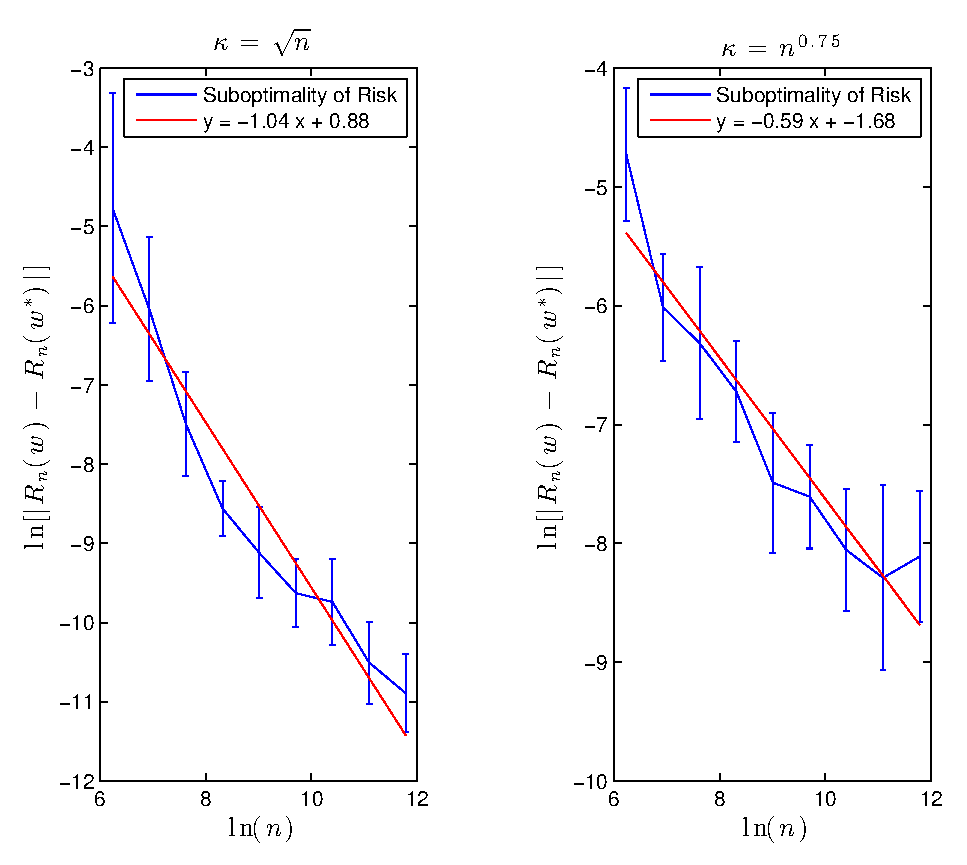
\includegraphics[width=0.8\textwidth]{slopes} 
\caption{The synatic }
\label{fig:slopes}
\end{figure}

 \begin{figure}
\center
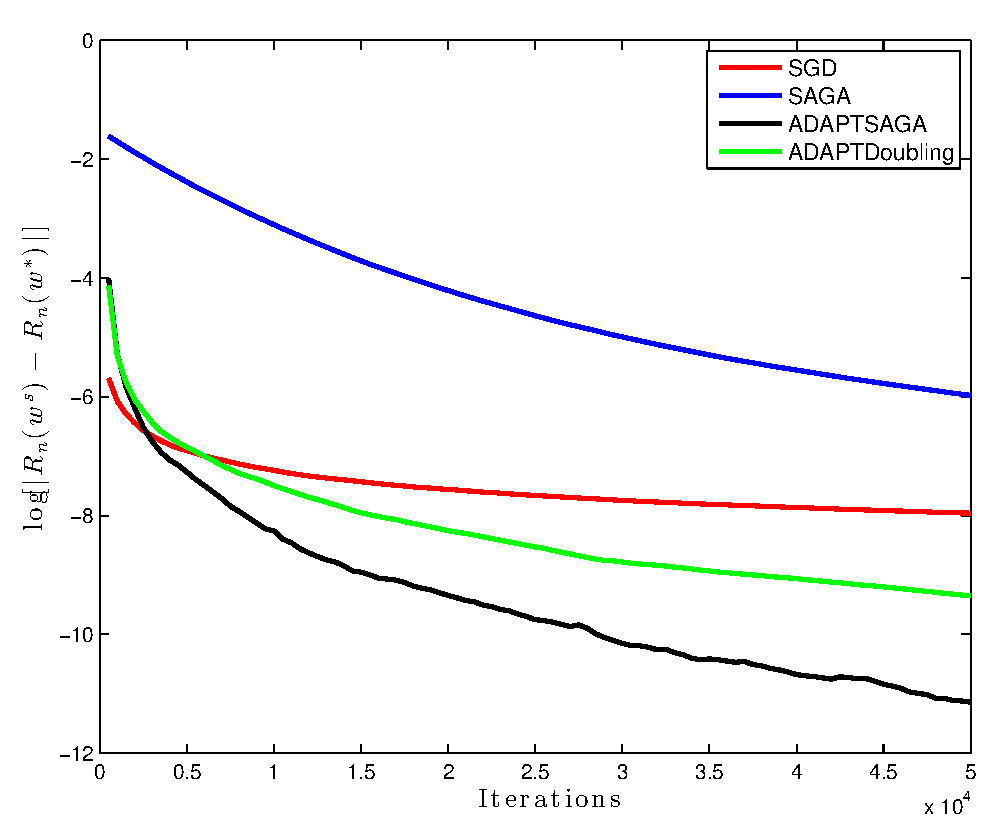
\includegraphics[width=0.5\textwidth]{ijcnn1} 
\caption{Test on ijcnn1 with step size $\eta = \frac{1}{3(\mu n + L)}$}
\label{fig:ijcnn1}
\end{figure}
\begin{figure}
\center
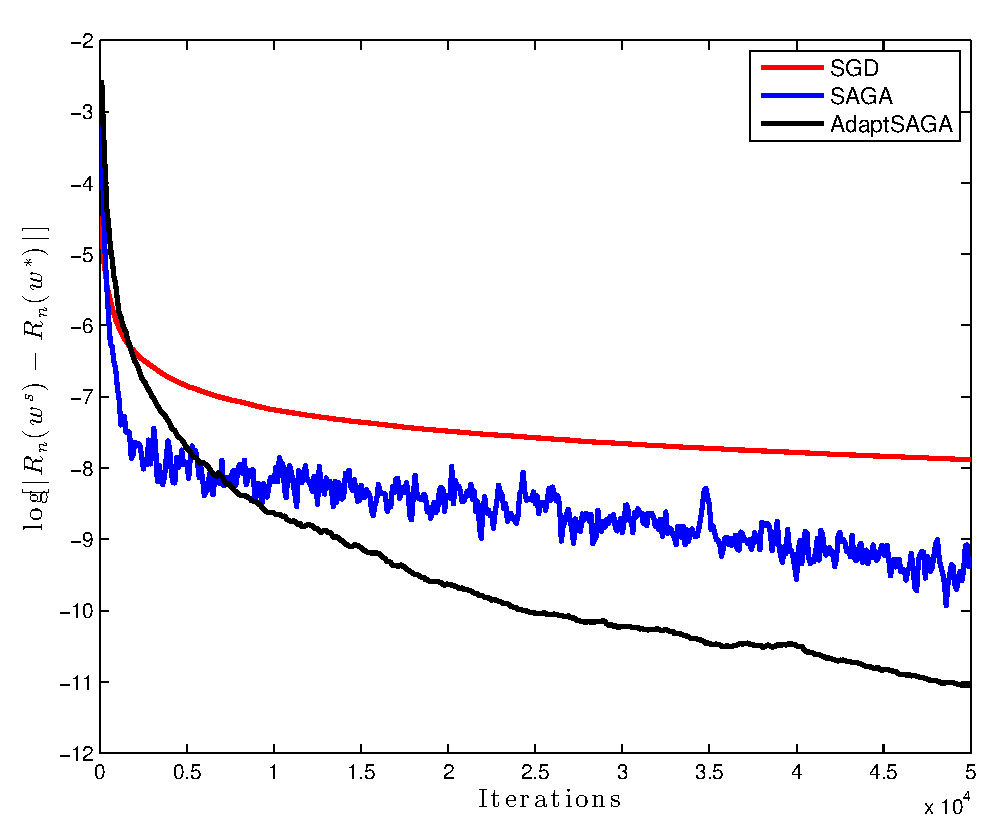
\includegraphics[width=0.5\textwidth]{ijcnn1_largestepsize} 
\caption{Test on ijcnn1 with step size $\eta = \frac{1}{3L}$}
\label{fig:ijcnn1_large}
\end{figure}
\begin{figure}
\center
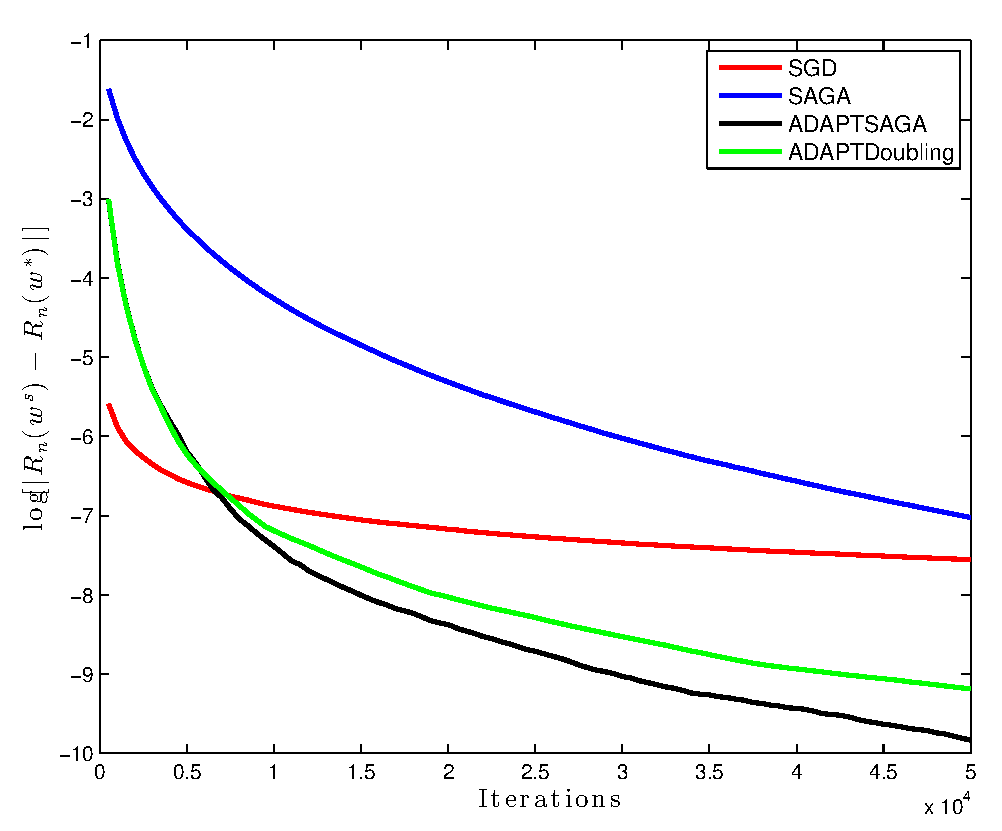
\includegraphics[width=0.5\textwidth]{wa} 
\caption{w8a dataset with $n = 49,749, d = 300$}
\label{fig:wa}
\end{figure}
\begin{figure}
\center
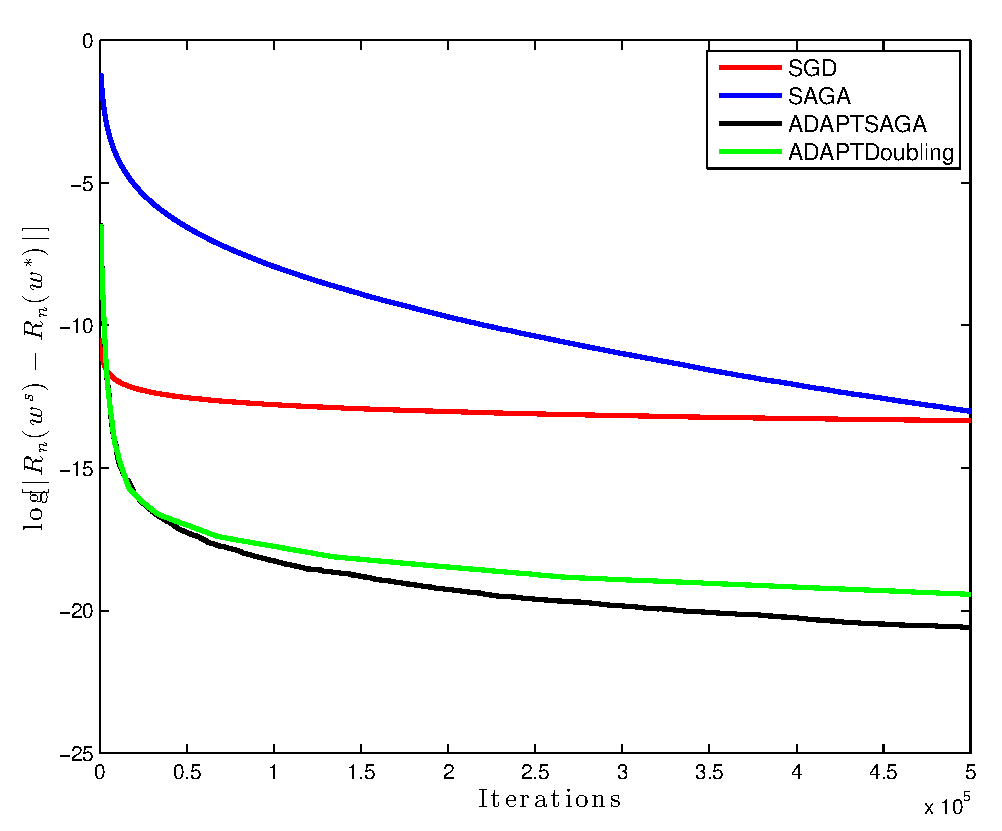
\includegraphics[width=0.5\textwidth]{covtype} 
\caption{covtype dataset with $n = 581,012, d = 54$}
\label{fig:covtype}
\end{figure}

\bibliographystyle{alpha}
\bibliography{bibliography}

\end{document}

